\begin{frame}{Introduction}
    \textbf{Where to find statistics data}\\
    \vspace{2em}
    Recently National Hockey League started they API service with stats data from 2010 year until present. API can be accessed publicly for free at: \textbf{statsapi.web.nhl.com/api/v1/endpoint\_name}\\
    \vspace{2em}
    This API operates on HTTP/S protocol and returns results in JSON format. Among others following statistics can be obtained from it:\\
    
    \begin{itemize}
        \item Game

        \item Team
        
        \item Player
    \end{itemize}
\end{frame} 

\begin{frame}{Introduction}
    \textbf{What statistics can be obtained}\\
    \vspace{2em}
    Following endpoints are available:
    
    \begin{description}
        \item[/conferences]     Get all current NHL conferences,
        \item[/divisions] 	    Get all current NHL divisions,
        \item[/draft] 	        Get round-by-round data for current year's NHL Entry Draft,
        \item[/game] 	        Get stats for an NHL game,
        \item[/people] 	        Get an NHL player,
        \item[/schedule] 	    Get the NHL game schedule,
        \item[/standings] 	    Get NHL division standings,
        \item[/standingsTypes] 	Get all available NHL standing types,
        \item[/statTypes]       Get all available NHL statistic types,
        \item[/teams] 	        Get all NHL teams.
    \end{description}
\end{frame}

\begin{frame}{Introduction}
    \textbf{How does NHL game look}\\
    \vspace{2em}
    \begin{itemize}
        \item 5 vs 5 game, 4 skaters, 1 goaltender
        \item 3 periods of 20 minutes
        \item game that ends with a tie goes into 5 minute sudden-death overtime
        \item shootouts happen after overtime in 3 round if tie remains, shootout continues until one team fails attempt of other
    \end{itemize}
\end{frame}

\begin{frame}{Introduction}
    \textbf{What are player positions}\\
    \vspace{2em}
    \begin{figure}[H]
        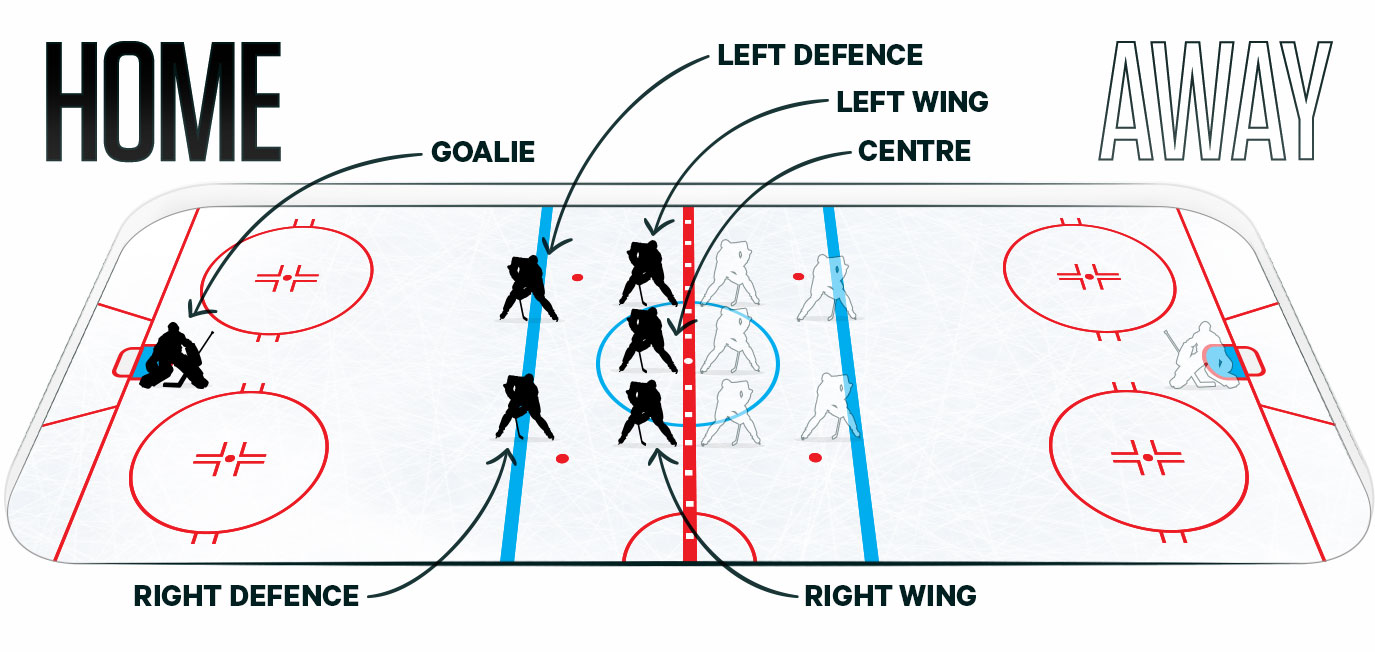
\includegraphics[width=\textwidth]{positions}
    \end{figure}
\end{frame}

\begin{frame}{Introduction}
    \textbf{What are player positions}\\
    \vspace{2em}
    \begin{itemize}
        \item goalie
        \item left defence
        \item right defence
        \item left wing
        \item centre
        \item right wing
    \end{itemize}
\end{frame}
